\section{Resultados e Discussões} \label{pontosResultados}

Como exposto nas Seções \ref{pontosProposta} e \ref{pontosBaseImg}, foi feita a obtenção de nuvens de pontos das bases de imagens utilizando três procedimentos:

\begin{enumerate}
\item \textbf{Método convencional}: Método no qual o usuário seleciona manualmente o conjunto de imagens mais bem expostas para assim gerar a nuvem de pontos.

\item \textbf{Método HDR}: Método no qual é utilizado um conjunto de imagens HDR \textit{tonemapped}, para obtenção da nuvem de pontos.

\item \textbf{Método proposto}: Trata-se de uma extensão do anterior, cujo diferencial é o realce dos contornos das imagens HDR \textit{tonemapped} antes de gerar a nuvem de pontos.
\end{enumerate}

Para isso, primeiramente foram geradas as imagens HDR, das base de imagens, utilizando o método proposto por Sen~\etal~\cite{hdrMovimento}. As imagens HDR resultantes são mostradas nas Figuras \ref{figResTonemap} e \ref{figRes2Tonemap} (representadas já com aplicação do \textit{tone mapping}, como definido na Seção~\ref{pontosToneMapping}). 

%É possível notar que as imagens HDR da Figura \ref{figRes2Tonemap} possuem distorção mais acentuada do cenário ao fundo, em relação às imagens da Figura \ref{figResTonemap}. Isso deve ocorrer devido ao maior desalinhamento existente entre imagens capturadas manualmente.

\begin{figure}[H]
  \centering 
  \subfloat[Objeto visto de frente.]
  {
    \includegraphics[height=5cm]{Base1/ToneMap/4}
    \label{figResTonemapA}
  }  
  \quad %espaco separador
  \subfloat[Objeto visto pela esquerda.]
  {
    \includegraphics[height=5cm]{Base1/ToneMap/3}
    \label{figResTonemapB}
  }
  \quad %espaco separador
  \subfloat[Objeto visto por cima.]
  {
    \includegraphics[height=5cm]{Base1/ToneMap/2}
    \label{figResTonemapC}
  }
  \quad %espaco separador
  \subfloat[Objeto visto pela direita.]
  {
    \includegraphics[height=5cm]{Base1/ToneMap/1}
    \label{figResTonemapD}
  }
  \caption{Imagens HDR \textit{tonemapped} da base de dados obtida com tripé (Seção~\protect\ref{pontosBControl}).}
  \label{figResTonemap}
\end{figure}

\begin{figure}[H]
  \centering 
  \subfloat[Objeto visto de frente.]
  {
    \includegraphics[height=5cm]{Base2/ToneMap/3}
    \label{figRes2TonemapA}
  }  
  \quad %espaco separador
  \subfloat[Objeto visto pela esquerda.]
  {
    \includegraphics[height=5cm]{Base2/ToneMap/2}
    \label{figRes2TonemapB}
  }
  \quad %espaco separador
  \subfloat[Objeto visto por cima.]
  {
    \includegraphics[height=5cm]{Base2/ToneMap/4}
    \label{figRes2TonemapC}
  }
  \quad %espaco separador
  \subfloat[Objeto visto pela direita.]
  {
    \includegraphics[height=5cm]{Base2/ToneMap/1}
    \label{figRes2TonemapD}
  }
  \caption{Imagens HDR \textit{tonemapped} da base de dados registrada manualmente (Seção~\protect\ref{pontosBLivre}).}
  \label{figRes2Tonemap}
\end{figure}

Após a geração das imagens HDR \textit{tonemapped}, foi feito o realce dos contornos das mesmas como proposto na Seção \ref{pontosProposta}. Para isso foi implementado um programa em C++, utilizando bibliotecas do OpenCV para execução do filtro. Foi estabelecido um valor empírico de $\alpha = 0.3$, visando realçar os contornos sem introduzir ruído. As Figuras \ref{figResRealce} e \ref{figRes2Realce} mostram as imagens realçadas.

\begin{figure}[H]
  \centering 
  \subfloat[Objeto visto de frente.]
  {
    \includegraphics[height=5cm]{Base1/Realcado/1}
    \label{figResRealceA}
  }  
  \quad %espaco separador
  \subfloat[Objeto visto pela esquerda.]
  {
    \includegraphics[height=5cm]{Base1/Realcado/4}
    \label{figResRealceB}
  }
  \quad %espaco separador
  \subfloat[Objeto visto por cima.]
  {
    \includegraphics[height=5cm]{Base1/Realcado/3}
    \label{figResRealceC}
  }
  \quad %espaco separador
  \subfloat[Objeto visto pela direita.]
  {
    \includegraphics[height=5cm]{Base1/Realcado/2}
    \label{figResRealceD}
  }
  \caption{Imagens HDR \textit{tonemapped} realçadas da base de dados obtida com tripé (Seção~\protect\ref{pontosBControl}).}
  \label{figResRealce}
\end{figure}

\begin{figure}[H]
  \centering 
  \subfloat[Objeto visto de frente.]
  {
    \includegraphics[height=5cm]{Base2/Realcado/4}
    \label{figRes2RealceA}
  }  
  \quad %espaco separador
  \subfloat[Objeto visto pela esquerda.]
  {
    \includegraphics[height=5cm]{Base2/Realcado/3}
    \label{figRes2RealceB}
  }
  \quad %espaco separador
  \subfloat[Objeto visto por cima.]
  {
    \includegraphics[height=5cm]{Base2/Realcado/1}
    \label{figRes2RealceC}
  }
  \quad %espaco separador
  \subfloat[Objeto visto pela direita.]
  {
    \includegraphics[height=5cm]{Base2/Realcado/2}
    \label{figRes2RealceD}
  }
  \caption{Imagens HDR \textit{tonemapped} realçadas da base de dados registrada manualmente (Seção~\protect\ref{pontosBLivre}).}
  \label{figRes2Realce}
\end{figure}

Foi feita então a geração de nuvens de pontos com os três métodos citados, para cada uma das bases de imagens. E sendo assim, foi feita a reunião dos principais dados quantitativos relativos a cada um dos métodos. As Tabelas \ref{tabResultados} e \ref{tabResultados2} mostram a média de pontos de interesse que foram corretamente correspondidos por par de imagens ($M_c$), assim como o número de pontos 3D obtidos nas nuvens de pontos de cada abordagem ($N_p$), e a quantidade de câmeras que tiveram suas posições inferidas com sucesso ($N_c$). As Figuras \ref{figNuvemPontosA}, \ref{figNuvemPontosB},\ref{figNuvemPontosC}, \ref{figNuvemPontos2A}, \ref{figNuvemPontos2B} e \ref{figNuvemPontos2C} mostram as nuvens de pontos obtidas, para cada base de imagens.

\begin{table}[H]
  \centering
  \caption{Resultados obtidos com a geração das nuvens de pontos relativas à base de imagens obtida com tripé (Seção~\protect\ref{pontosBControl}).}
  \label{tabResultados}
  \begin{tabular}{l|l|l|l}
    \hline
               & $M_c$ &  $N_p$ & $N_c$ \\
    \hline
    Imagens LDR convencionais & 293,5 & 115 & 3 \\
    \hline
    Imagens \textit{tonemapped} & 291,16 & 732 & 4 \\  
    \hline
    Imagens \textit{tonemapped} & 306,6 & 1119 & 4 \\
    com realce de contornos & & & \\  
    \hline
  \end{tabular}
\end{table}

\begin{table}[H]
  \centering
  \caption{Resultados obtidos com a geração das nuvens de pontos relativas à base de imagens manual (Seção~\protect\ref{pontosBLivre}).}
  \label{tabResultados2}
  \begin{tabular}{l|l|l|l}
    \hline
               & $M_c$ &  $N_p$ & $N_c$ \\
    \hline
    Imagens LDR convencionais & 378 & 883 & 4 \\
    \hline
    Imagens \textit{tonemapped} & 368,3 & 900 & 4 \\  
    \hline
    Imagens \textit{tonemapped} & 363,3 & 906 & 4 \\
    com realce de contornos & & & \\  
    \hline
  \end{tabular}
\end{table}

Neste trabalho foram feitas apenas análises quantitativas sobre a aquisição das nuvens de pontos. Não foram feitas análises quanto a qualidade ou precisão dos pontos 3D gerados, pois para isso, seria necessário a existência de um modelo 3D de referência de alta precisão para comparação. E isso, por sua vez, exige o uso de equipamentos sofisticados que estão fora do alcance do projeto em questão.

Os resultados mostraram que, para as bases de imagens utilizadas, o uso de imagens HDR na geração de nuvem de pontos levou ao aumento no número de pontos 3D obtidos. Cada método proposto obteve os seguintes resultados em relação ao método convencional:

\begin{enumerate}
\item \textbf{Método HDR}: Para a base de dados obtida com tripé, este método apresentou um aumento de $536\%$ em número de pontos 3D obtidos em comparação ao método convencional. Já para a base de dados manual, apresentou um aumento de $1,9\%$ em número de pontos 3D obtidos.

\item \textbf{Método proposto}: Para a base de dados obtida com tripé, este método apresentou um aumento de $873\%$ em número de pontos 3D obtidos em comparação ao método convencional. Já para a base de dados manual, apresentou um aumento de $2,6\%$ em número de pontos 3D obtidos.
\end{enumerate}

Vale ressaltar que, além do aumento no número de pontos obtidos, o uso das imagens HDR possibilitou a inferência da posição das quatro câmeras da base de dados obtida com tripé. Já ao utilizar as imagens LDR convencionais, só foi possível inferir a posição de três das quatro câmeras. Isso pode ser visualizado na Figura \ref{figNuvemPontosA}.

\begin{figure}[H]
  \centering 
  \includegraphics[height=10cm]{Base1/ResultadosSFM/nuvemConvencional} 
  \caption{Nuvens de pontos obtida utilizando imagens LDR convencionais da base de imagens capturada com tripé.}
  \label{figNuvemPontosA}
\end{figure}

\begin{figure}[H]
  \centering 
  \includegraphics[height=10cm]{Base1/ResultadosSFM/nuvemToneMap}
  \caption{Nuvens de pontos obtida utilizando as imagens HDR \textit{tonemapped} da base de imagens capturada com tripé.}
  \label{figNuvemPontosB}
\end{figure}

\begin{figure}[H]
  \centering 
  \includegraphics[height=10cm]{Base1/ResultadosSFM/nuvemRealce}
  \caption{Nuvens de pontos obtida utilizando as imagens HDR \textit{tonemapped} com realce de contornos da base de imagens capturada com tripé.}
  \label{figNuvemPontosC}
\end{figure}

\begin{figure}[H]
  \centering 
  \includegraphics[height=10cm]{Base2/ResultadosSFM/nuvemConvencional}
  \caption{Nuvens de pontos obtida utilizando imagens LDR convencionais da base de imagens capturada manualmente.}
  \label{figNuvemPontos2A}
\end{figure}

\begin{figure}[H]
  \centering 
  \includegraphics[height=10cm]{Base2/ResultadosSFM/nuvemToneMap}
  \caption{Nuvens de pontos obtida utilizando as imagens HDR \textit{tonemapped} da base de imagens capturada manualmente.}
  \label{figNuvemPontos2B}
\end{figure}

\begin{figure}[H]
  \centering 
  \includegraphics[height=10cm]{Base2/ResultadosSFM/nuvemRealce}
  \caption{Nuvens de pontos obtida utilizando as imagens HDR \textit{tonemapped} com realce de contornos da base de imagens capturada manualmente.}
  \label{figNuvemPontos2C}
\end{figure}